\documentclass[letterpaper]{article}
\usepackage{natbib,alifeconf}
\usepackage{hyperref}


\usepackage[flushleft]{threeparttable}
\usepackage{subcaption}
\usepackage{booktabs}
\setcounter{tocdepth}{3}
\usepackage{array}
\usepackage{float}

\title{Heterogeneous Cellular Automata Evolution in a Fluctuating Environment}
\author{First Author$^{1}$, Second Author$^{1,2}$, Third Author$^{1,2}$, Fourth Author$^{1,2}$ \and Fifth Author$^2$ \\
\mbox{}\\
$^1$First affiliation  \\
$^2$Second affiliation \\
corresponding@author.email}


\begin{document}
\maketitle

\begin{abstract}
The importance of environnemental fluctuations in the evolution of living beings by natural selection have been widely noted by biologists and have been linked to many important characteristics of the life as: modularity, plasticity, size of the genotype, mutation rate, learning or epigenetic adaptations. However, in artificial life simulations, environmental fluctuations are usually seen as a problem to be solved rather than an essential characteristic of evolution. We propose in this paper to use HetCA, an heterogeneous cellular automata characterized by its ability to generate open ended long-term evolution and evolutionary progress, to measure the impact of different forms of environmental fluctuations. Our results indicate that environnemental fluctuations induce mechanisms analogous to epigenetic adaptations in HetCA.
\end{abstract}



\section{Introduction}
If early population genetics theory assumed the environment to be constant, since Richards Levins works \cite{levins1968evolution} in the 70's up to Evolution in Four Dimensions by Eva Jablonka and al. \cite{jablonka2014evolution} the importance of environnemental fluctuations in the evolution of living beings by natural selection have been widely noted. Through those works and others, environmental fluctuations have been linked to many important questions about the mechanisms of evolution such as: modularity, plasticity, size of the genotype, mutation rate and through this the evolvability. Recently Jablonka\cite{jablonka2014evolution} have developed the idea that epigenetic mechanisms controlling the rate of changes in certain genes have evolved to counter frequent environmental changes. 
Environmental changes can include introduction of new predator or new potencial food, radical environment modifications such as climate change inducing environmental stress but also cyclic changes such as daily cycle of light and darkness, seasons...  

In \cite{lachmann1996inheritance} Lachemann model the consequences of such cycling variations on phenotypical inheritances. Their model predict that, when those cycles are longer than the reproductive cycle but relatively short heritable variations produced by non-DNA inheritance systems are likely to be observed.

Many work in artificial life approach the issue of environmental variations especially in evolutionary robotics\cite{floreano2000evolutionary}, but the greater part are interested mainly in the spacial variations, or considering them as a problem to solve.

This paper is organized as follows. Section 2 highlights consequences of variable environment in biological evolution. In Section 3, we explain the mecanisms of HetCA simulation. The implementation of environmental fluctuation in HetCA  is then explained in Section 4. Section 5 details the computer experimental setup while we reports experimental results in Section 6. We discuss the implications of these results in Section 7. Finally, Section 8 concludes the paper.


\section{Background}
In \cite{lipson2002origin} Lipson demonstrated a correlation between the modularity and the rate of change of the environment resources. While in \cite{yu2007program} Yu used  observed populations exploit neutrality to cope with environmental fluctuations and therefore evolve some sort of evolvability under 2 alternating objective functions. Both simulations used Genetic Programming (GP) and explicit fitness functions.

\section{HetCA}
HetCA is based on classical two-dimensional CA, to which it added the following features : Cells have "age", "decay", and "quiescence" properties; cells utilize a heterogeneous transition function inspired by linear genetic programming; and there exists a notion of genetic transfer of transition functions between adjacent cells
HetCA exhibit longterm phenotypic dynamics, sustaining a high level of variance
over very long runs and displayed greater behavioral diversity than classical cellular automata\cite{medernach2013long}. HetCA also display Shanahan \cite{shanahan2012evolutionary} definition of evolutionary progress on three criteria: robustness, size and density of generated genotypes\cite{medernach2015evolutionary}.

Moreover, some emergent properties of HECA are similar to two of the five major eukaryotic innovations which do not appear to
have direct prokaryotic predecessors defined in~\cite{smith1997major} as : the eukaryotic chromatin remodeling machinery; the cell cycle regulation
systems; the nuclear envelope, the cytoskeleton; and the apoptosis apparatus\cite{koonin2002origin}. Indeed, in HetCA, the loss of the genotype of the cell as it turns to the quiescent state may seem similar to apoptosis while survival strategies such as the ones depicted in Figure~\ref{foursteps} might akin cell cycle regulation systems. 

\section{Experimental Setup}
\subsection{Environmental Fluctuations}
Originally, in HetCA, the new genotype of a cell was randomly chosen among candidates genotypes. To introduce environmental variations, we chose to vary the likelihood of spread of the genotype of a cell according to the state of this cell. The chances of the candidate genotype of the cell $c$ to be selected are then: $c=K(S_c)/\sum_{i=1}^{n} K(S_{c_i})$ with $S_c$ state of the cell $c$, $K(S)$ likelihood of spread of state $S$ and $n$ number of candidate genotypes. Therefore an environment is characterized by the odds of propagation of the five living states $\{K(S_1),K(S_2),K(S_3),K(S_4),K(S_5)\}$.   
To mimic environmental fluctuations we initialise the simulation with $K(S_i)=1  \forall i \in [1,5]$ and then we regularly change those values from iteration 3000 of the cellular automata. 

We chose to introduce four forms of environmental fluctuations described in Table~\ref{tab:environments}.

\noindent The \emph{Short-cycle Fluctuation} : consists of alternating between two environments every 100 iterations of the cellular automaton. We chose to vary the environment every 100 iterations to stay in the same range of frequency as in Lispson \cite{lipson2002origin} examples 20 and 100 generations and \cite{yu2007program} experiments 10, 20 and 50 generations. In fact we consider that a successful reproductive cycle involves passing a cell through the quiescent state. And this should takes between two iterations (alternating between the quiescent state and a living state) and seven iterations  (if a cell remains in a living state more than seven consecutive iterations it goes to the decay state and can not receive genotype for an important period).

\noindent The \emph{Light Fluctuation} : consists of alternating between five environments every 5000 iterations of the cellular automaton. The first fives each prohibit a different state from the five living state, the latter gives equal chance to each of the five states.

\noindent The \emph{Strong Fluctuation} : consists of alternating between twelve environments every 5000 iterations of the cellular automaton. The first eleven each prohibit a different combination of two states from the five living state, the latter gives equal chance to each of the five states.

\noindent The \emph{Gradual Fluctuation} : is similar to the strong fluctuation except that it include a transition phase of $T=60$ iterations in between two environment where spread likehood values progressively switch from the value a previous environment to the ones of the new environment. Over this phase the sate spreading is defined by the following formula : $K(S,t)=K_p(S) \times (T-t) + K_{p+1}(S) \times t$ where $t$ is the number of iteration achieved since the beginning of the transition phase; $K_p(S)$ and $K_{p+1}(S)$ are likelihood of spread of state $S$ for the curent environment and the next environment. 


Owing to the variety of biological temporal rhythms and reproductive cycles the relevance of the following analogy is certainly limited . However \emph{short-cycle fluctuation} would be similar to what are the circadian rhythms for some bacteria: very regular cycles in which these organisms have enough time to reproduce several times. While \emph{light fluctuation} would be closer to seasonal fluctuations and \emph{strong and gradual fluctuations} would akin ecological crisis. 

\subsection{Common Settings}
For each forms of environmental fluctuations plus the stable non fluctuating environment, we performed 50 simulations, each on 500000 iterations with the parameters listed in Table~\ref{settings}. The genotypes of an individual are its transition rules encoded with CA-LGP using the function set depicted in Table~\ref{funcSet}. Mutation of genotypes is enabled and we use the Micro/Marco-mutation of CA-LGP described in \cite{medernach2013long}.



\begin{table}
\scriptsize
\centering
\begin{tabular}{l>{\centering}p{0.2\columnwidth}}\toprule%
Parameter & Value \tabularnewline
\toprule%
Number of living states & 5\tabularnewline
Successive living iterations before decay & 7\tabularnewline
Number of iterations for decay & 375-1875\tabularnewline
Direct transition to decay & enabled\tabularnewline
Size of the grid & 500x500\tabularnewline
Grid boundaries & toric grid\tabularnewline
Transition Rule~(TR) & CA-LGP\tabularnewline
Maximum (TR) size & 50 program statements\tabularnewline
Genotype copy neighboring  & Von Neumann \tabularnewline
Transition rule neighboring & Moore\tabularnewline
\bottomrule%
\end{tabular}
\caption{ \textbf{HetCA parameters}.}
  \label{settings}
\end{table}


\begin{table}
\scriptsize
\centering
  \begin{tabular}{l>{\centering}p{0.6\columnwidth}}
  \toprule%
    \textbf{op. name}	& \textbf{action} on inputs $(x,y)$\tabularnewline
 \toprule%   
    abs			& $|x|$ \tabularnewline
    plus		& $x+y$ \tabularnewline
    delta		& 1, if $|x-y| < 1/10000$; 0 o.w. \tabularnewline
    dist		& $|x-y|$ \tabularnewline
    inv			& $1-x$ \tabularnewline
    inv2		& safeDiv($1, x$) \tabularnewline
    magPlus		& $|x+y|$ \tabularnewline
    max			& $\max \{x,y\}$ \tabularnewline
    min			& $\min \{x,y\}$ \tabularnewline
    safeDiv		& $x/y$ if $|y| >  1/10000$; 1 o.w. \tabularnewline
    safePow		& $x^y$, if defined; 1 o.w. \tabularnewline
    thresh		& 1, if $x > y$; 0 o.w.\tabularnewline
    times		& $xy$ \tabularnewline
    zero		& 1, if $|x| < 1/10000$; 0 o.w. \tabularnewline
\bottomrule%
  \end{tabular}
    \caption{\textbf{Function set}. \label{funcSet}}
\end{table}

\section{Methodology}

\subsection{Genotype Size}
We use the number of program statements ($n_{prog}$) as a measure of the genotype size. We compute the average size of all the current genotypes of a run every 2500 iterations. We then report the average and standard error among all the fifty runs sharing the same settings.

\subsection{Changes induces by environmental fluctuation}
To measure the impact of environmental fluctuations on the phenotypes we compare, for each run, their data at iteration $t$ with that at iteration $t + 5000$ ($t + 7500$ for \emph{Short-cycle Fluctuation}).

\subsection{Density}
We also collect the \emph{most common genotype}~(most frequently occurring) in iterations 2500\footnote{\cite{medernach2015evolutionary}  has shown that the most common genotypes during the first iterations of HetCA were unlikely to have a viable survival strategy, therefore we chose to collect genotypes from iteration 2500.}, 102500, 202500, 302500, 402500 and 500000. 

\subsection{Regularities measurement}
In HetCA to survive in the long term, the genotypes must regularly release cells by transforming them into quiescent cells without genotypes. This generates patterns and cycles quite easy to observe in homogeneous simulations where a single genotype is tested, Figure~\ref{foursteps} but also observable although with more difficulties in normal, heterogeneous, HetCA simulations Figure~\ref{fourstepsreal}. That is why we found it useful to measure these cycles as well as out-of regularities. If the genotype of a cell use a stable strategy, i.e. a sequence of states being repeated, this sequence must contain a minimum of two state to ensure the survival of the genotype, the quiescent state and one of the living state.  
 
\begin{figure}[h]
\centering
\includegraphics[width=0.75\columnwidth]{4steptransition}
\caption{\textbf{Six steps survival strategy} from a genotype extracted from an HetCA simulation in a stable environment and tested here in a randomly initialized homogenous CA. }
  \label{foursteps}
\end{figure}
 
\begin{figure}[h]
\centering
\includegraphics[width=0.75\columnwidth, angle =-90]{cyclesReal}
\caption{\textbf{Six steps survival strategy} from an HetCA simulation with \emph{Short-cycle Fluctuation}. }
  \label{fourstepsreal}
\end{figure}

$\min k \in [2;7], S_t=S_{t-k} \wedge S_{t-1}=S_{t-1-k}$ where $S_t$  is the state of the considered cell at iteration $t$.
For this, at every iteration of the cellular automata, we compare the state of each cell to their state during the eight previous iterations of the CA. We then measure whether a sequence of states is repeated during these eight iterations.


\newcommand*{\TitleParbox}[1]{\parbox[l]{10cm}{\raggedright #1}}%
\begin{table*}
\caption{Environments.\label{tab:environments}}
\scriptsize

\begin{tabular}{lccccl}
\toprule%
{\textbf{Name}} & {\textbf{Short Name}} & \textbf{Cycles}\tnote{a} & \textbf{Transitions}\tnote{b} &\textbf{Environment list} \tabularnewline
\toprule%
\textbf{Stable Environment} & [SE] & NA & NA & \TitleParbox{$\{1,1,1,1,1\}$} \tabularnewline

\textbf{Short-cycle Fluctuations} & [ScF] & 100 & 1 & \TitleParbox{$\{1,1,1,0,0\}$, $\{1,1,1,0,0\}$} \tabularnewline

\textbf{Light Fluctuations} & [LF] & 5000 &  1 & \TitleParbox{$\{1,1,1,1,0\}$, $\{1,1,1,0,1\}$, $\{1,1,0,1,1\}$, $\{1,0,1,1,1\}$, $\{0,1,1,1,1\}$, $\{1,1,1,1,1\}$}\tabularnewline
    
\textbf{Strong Fluctuations} & [SF] & 5000 & 1 & \TitleParbox{$\{0,0,1,1,1\}$, $\{1,1,1,0,0\}$, $\{0,1,0,1,1\}$, $\{1,0,1,1,0\}$, $\{0,1,1,0,1\}$, $\{1,1,0,1,0\}$, $\{1,0,1,0,1\}$, $\{0,1,1,1,0\}$, $\{1,0,0,1,1\}$, $\{1,1,0,0,1\}$, $\{1,1,1,1,1\}$} \tabularnewline

\textbf{Gradual Fluctuations} & [GF] & 5000  & 60 & \TitleParbox{$\{0,0,1,1,1\}$, $\{1,1,1,0,0\}$, $\{0,1,0,1,1\}$, $\{1,0,1,1,0\}$, $\{0,1,1,0,1\}$, $\{1,1,0,1,0\}$, $\{1,0,1,0,1\}$, $\{0,1,1,1,0\}$, $\{1,0,0,1,1\}$, $\{1,1,0,0,1\}$, $\{1,1,1,1,1\}$} \tabularnewline

\bottomrule%
\end{tabular}%
\end{table*} 



\section{Results}
\begin{figure}[h]
\centering
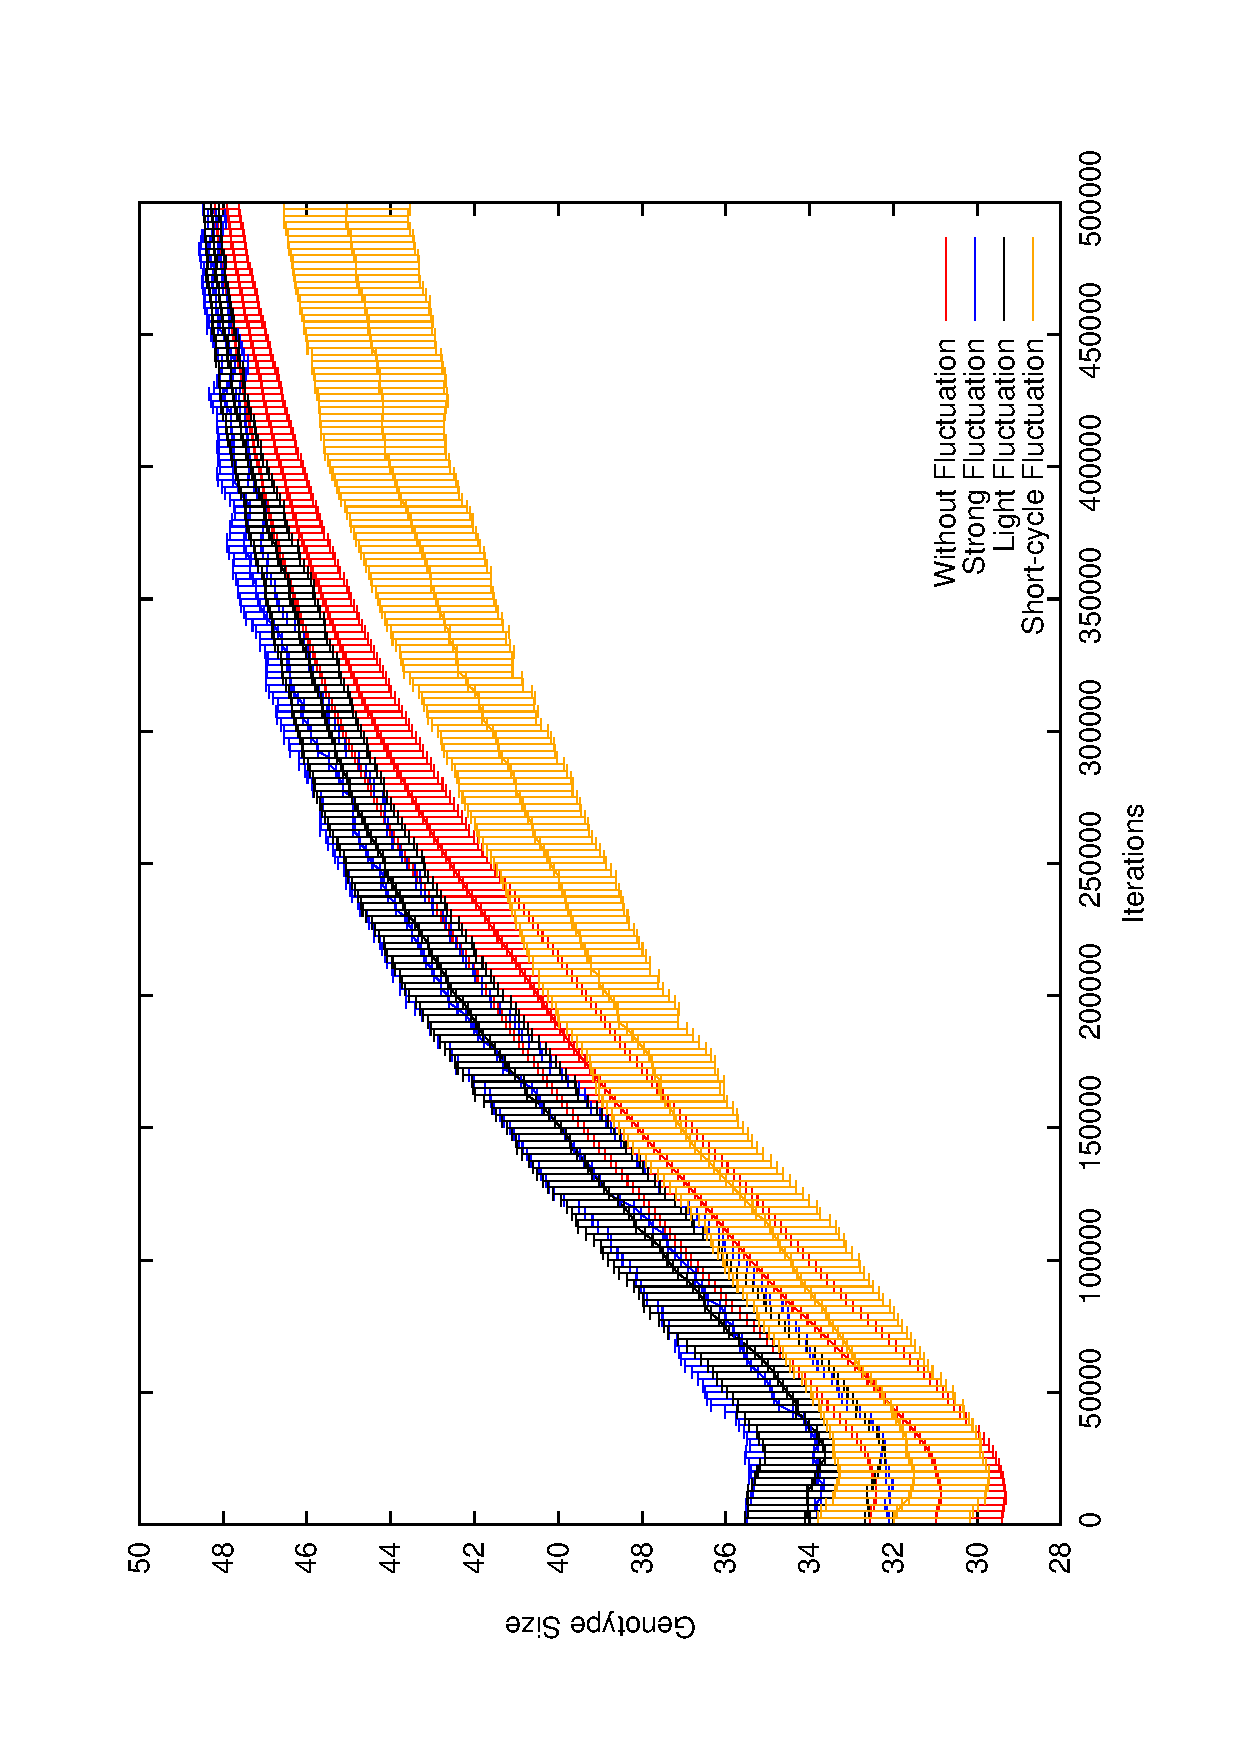
\includegraphics[width=0.7\columnwidth, angle =-90 ]{Size}
\caption{\textbf{Size of genotypes}. The size is bounded (50 is the maximum size) and  it probably limits the differences, however, one can clearly see here that \emph{Short-cycle  Fluctuation} restrict the size of the genotypes while other forms of fluctuations do not restrict or even increase it.
}
\label{Size}
\end{figure}

\begin{figure}[h]
\centering
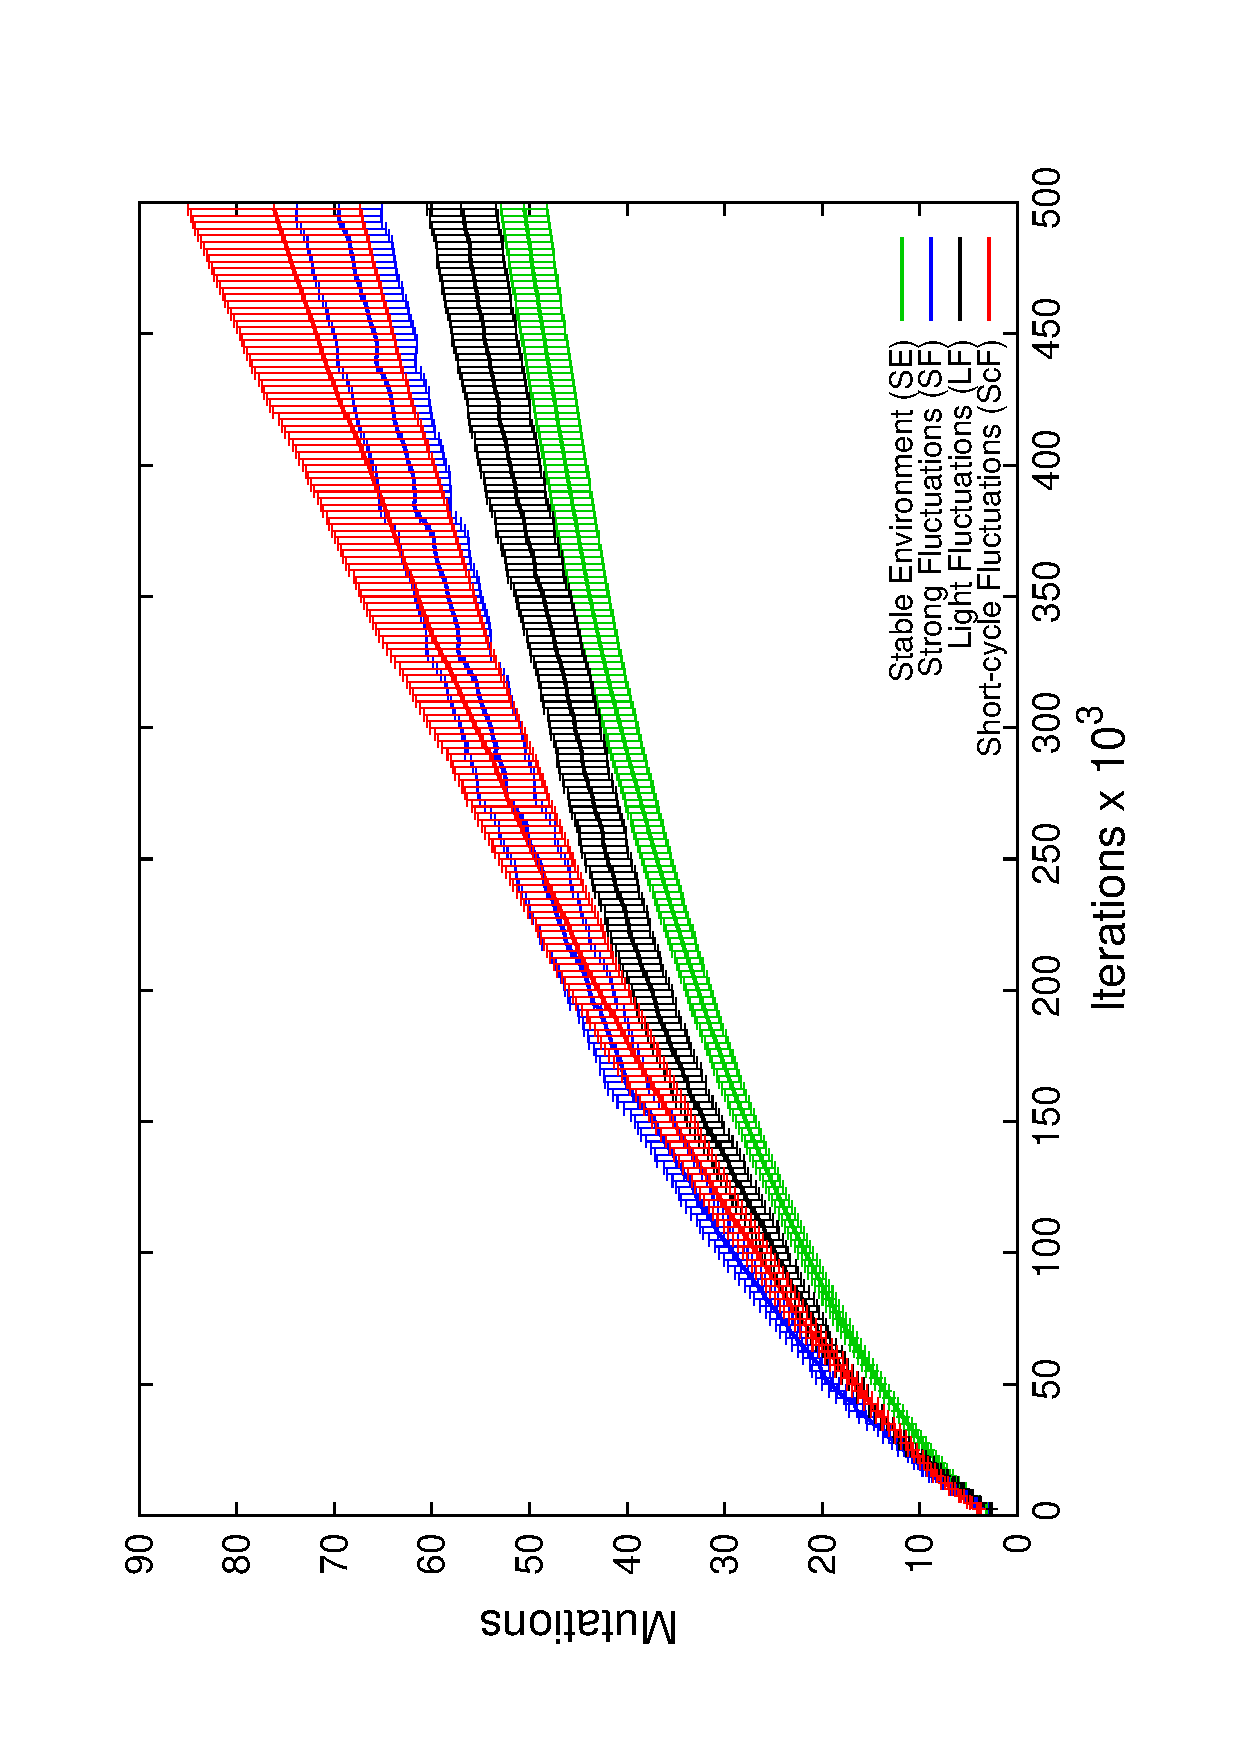
\includegraphics[width=0.7\columnwidth, angle =-90 ]{Mutations}
\caption{\textbf{Mutations of genotypes}.
}
\label{Mutations}
\end{figure}

\begin{figure}[h]
\centering
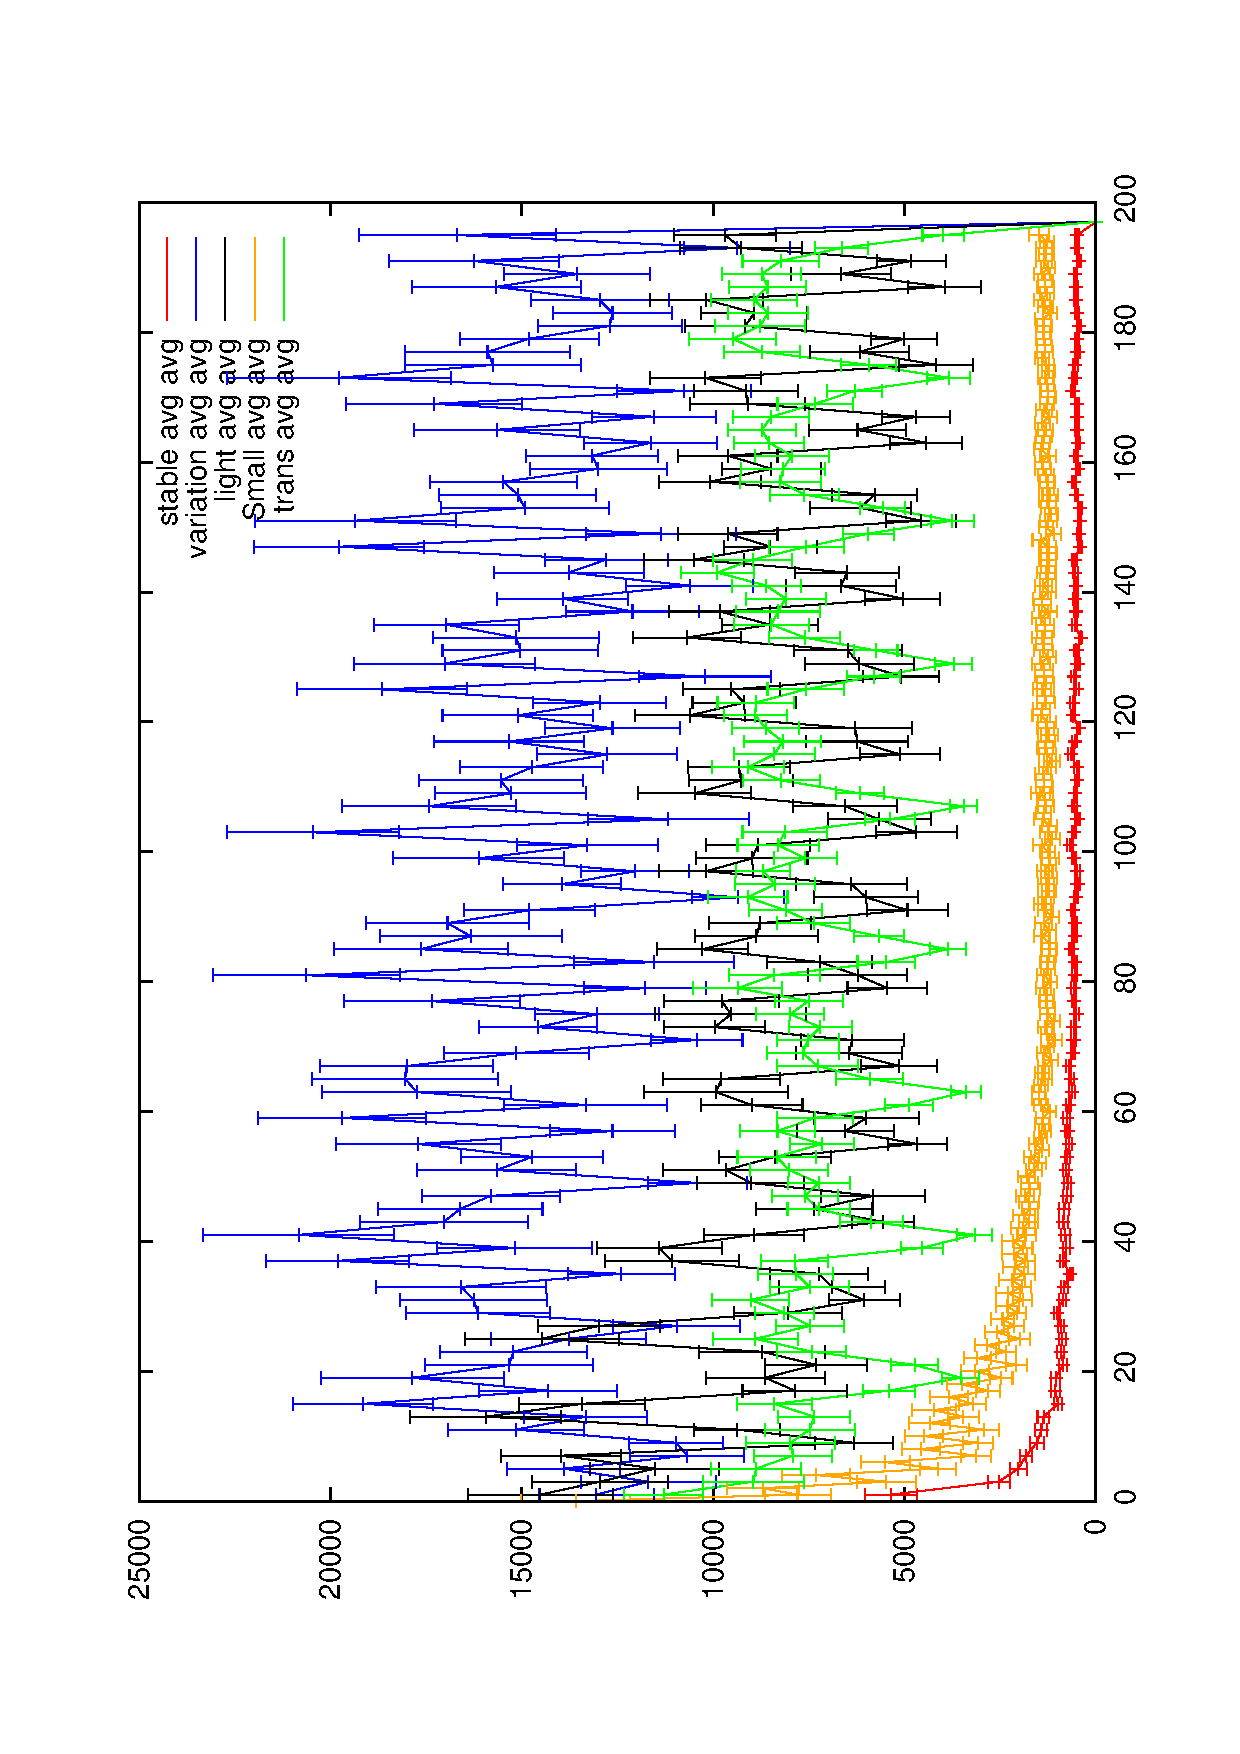
\includegraphics[width=0.7\columnwidth, angle =-90 ]{cumuldiff}
\caption{\textbf{Changes} : Here one can see that the impact of environmental fluctuations decreases for \emph{Short-cycle  Fluctuation} while it remains very high for other forms of environmental fluctuations.
}
\label{Mutations}
\end{figure}

\begin{figure}[H]
\begin{subfigure}{.25\textwidth}
  \centering
  \includegraphics[width=.7\linewidth, angle =-90]{boxdensitystable.eps}
  \caption{Stable environment.}
  \label{fig:sfig1}
\end{subfigure}%
\begin{subfigure}{.25\textwidth}
  \centering
  \includegraphics[width=.7\linewidth, angle =-90]{boxdensityvariation.eps}
  \caption{Strong Fluctuation.}
  \label{fig:sfig2}
\end{subfigure}

\begin{subfigure}{.25\textwidth}
  \centering
  \includegraphics[width=.7\linewidth, angle =-90]{boxdensityvariationLight.eps}
  \caption{Light Fluctuation.}
  \label{fig:sfig2}
\end{subfigure}%
\begin{subfigure}{.25\textwidth}
  \centering
  \includegraphics[width=.7\linewidth, angle =-90]{boxdensityvariationSmall.eps}
  \caption{Small Fluctuation.}
  \label{fig:sfig1}
\end{subfigure}
\caption{Density of Genotype : Each genotype density is processed in four possible different environments.}
\label{fig:size}
\end{figure}

\begin{figure}[H]
\begin{subfigure}{.25\textwidth}
  \centering
  \includegraphics[width=.7\linewidth, angle =-90]{boxendingsFailedstable.eps}
  \caption{Stable environment.}
  \label{fig:sfig1}
\end{subfigure}%
\begin{subfigure}{.25\textwidth}
  \centering
  \includegraphics[width=.7\linewidth, angle =-90]{boxendingsFailedvariation.eps}
  \caption{Strong Fluctuation.}
  \label{fig:sfig2}
\end{subfigure}

\begin{subfigure}{.25\textwidth}
  \centering
  \includegraphics[width=.7\linewidth, angle =-90]{boxendingsFailedvariationLight.eps}
  \caption{Light Fluctuation.}
  \label{fig:sfig2}
\end{subfigure}%
\begin{subfigure}{.25\textwidth}
  \centering
  \includegraphics[width=.7\linewidth, angle =-90]{boxendingsFailedvariationSmall.eps}
  \caption{Small Fluctuation.}
  \label{fig:sfig1}
\end{subfigure}
\caption{Last iteration with living cells of density runs that didn't reach 60000 iterations. Note that \emph{Short-cycle Fluctuation} genotypes failures are concentrated around iteration 15000 on \emph{Light Fluctuation} density test and around iteration 25000 on \emph{Strong Fluctuation} density test.}
\label{fig:size}
\end{figure}

\section{Discussions}

\section{Qualitative Analysis}


\section{Conclusions}
\bibliography{gp-bibliography,David}{}

\bibliographystyle{plain}
\bibliographystyle{abbrv}
\end{document}
